\PassOptionsToPackage{unicode=true}{hyperref} % options for packages loaded elsewhere
\PassOptionsToPackage{hyphens}{url}
\PassOptionsToPackage{dvipsnames,svgnames*,x11names*}{xcolor}
%
\documentclass[11pt,a4paper,krantz2,11pt,oneside]{krantz}
\usepackage{lmodern}
\usepackage{amssymb,amsmath}
\usepackage{ifxetex,ifluatex}
\usepackage{fixltx2e} % provides \textsubscript
\ifnum 0\ifxetex 1\fi\ifluatex 1\fi=0 % if pdftex
  \usepackage[T1]{fontenc}
  \usepackage[utf8]{inputenc}
  \usepackage{textcomp} % provides euro and other symbols
\else % if luatex or xelatex
  \usepackage{unicode-math}
  \defaultfontfeatures{Ligatures=TeX,Scale=MatchLowercase}
    \setmainfont[]{Alegreya}
\fi
% use upquote if available, for straight quotes in verbatim environments
\IfFileExists{upquote.sty}{\usepackage{upquote}}{}
% use microtype if available
\IfFileExists{microtype.sty}{%
\usepackage[]{microtype}
\UseMicrotypeSet[protrusion]{basicmath} % disable protrusion for tt fonts
}{}
\IfFileExists{parskip.sty}{%
\usepackage{parskip}
}{% else
\setlength{\parindent}{0pt}
\setlength{\parskip}{6pt plus 2pt minus 1pt}
}
\usepackage{xcolor}
\usepackage{hyperref}
\hypersetup{
            pdftitle={Memoire de mise en situation professionnel --- Créer une bibliothèque PHP},
            pdfauthor={Germain Jr.~OLEA-OYOUGOU},
            colorlinks=true,
            linkcolor=Maroon,
            filecolor=Maroon,
            citecolor=Blue,
            urlcolor=Blue,
            breaklinks=true}
\urlstyle{same}  % don't use monospace font for urls
\usepackage{color}
\usepackage{fancyvrb}
\newcommand{\VerbBar}{|}
\newcommand{\VERB}{\Verb[commandchars=\\\{\}]}
\DefineVerbatimEnvironment{Highlighting}{Verbatim}{commandchars=\\\{\}}
% Add ',fontsize=\small' for more characters per line
\usepackage{framed}
\definecolor{shadecolor}{RGB}{248,248,248}
\newenvironment{Shaded}{\begin{snugshade}}{\end{snugshade}}
\newcommand{\AlertTok}[1]{\textcolor[rgb]{0.33,0.33,0.33}{#1}}
\newcommand{\AnnotationTok}[1]{\textcolor[rgb]{0.37,0.37,0.37}{\textbf{\textit{#1}}}}
\newcommand{\AttributeTok}[1]{\textcolor[rgb]{0.61,0.61,0.61}{#1}}
\newcommand{\BaseNTok}[1]{\textcolor[rgb]{0.06,0.06,0.06}{#1}}
\newcommand{\BuiltInTok}[1]{#1}
\newcommand{\CharTok}[1]{\textcolor[rgb]{0.5,0.5,0.5}{#1}}
\newcommand{\CommentTok}[1]{\textcolor[rgb]{0.37,0.37,0.37}{\textit{#1}}}
\newcommand{\CommentVarTok}[1]{\textcolor[rgb]{0.37,0.37,0.37}{\textbf{\textit{#1}}}}
\newcommand{\ConstantTok}[1]{\textcolor[rgb]{0,0,0}{#1}}
\newcommand{\ControlFlowTok}[1]{\textcolor[rgb]{0.27,0.27,0.27}{\textbf{#1}}}
\newcommand{\DataTypeTok}[1]{\textcolor[rgb]{0.27,0.27,0.27}{#1}}
\newcommand{\DecValTok}[1]{\textcolor[rgb]{0.06,0.06,0.06}{#1}}
\newcommand{\DocumentationTok}[1]{\textcolor[rgb]{0.37,0.37,0.37}{\textbf{\textit{#1}}}}
\newcommand{\ErrorTok}[1]{\textcolor[rgb]{0.14,0.14,0.14}{\textbf{#1}}}
\newcommand{\ExtensionTok}[1]{#1}
\newcommand{\FloatTok}[1]{\textcolor[rgb]{0.06,0.06,0.06}{#1}}
\newcommand{\FunctionTok}[1]{\textcolor[rgb]{0,0,0}{#1}}
\newcommand{\ImportTok}[1]{#1}
\newcommand{\InformationTok}[1]{\textcolor[rgb]{0.37,0.37,0.37}{\textbf{\textit{#1}}}}
\newcommand{\KeywordTok}[1]{\textcolor[rgb]{0.27,0.27,0.27}{\textbf{#1}}}
\newcommand{\NormalTok}[1]{#1}
\newcommand{\OperatorTok}[1]{\textcolor[rgb]{0.43,0.43,0.43}{\textbf{#1}}}
\newcommand{\OtherTok}[1]{\textcolor[rgb]{0.37,0.37,0.37}{#1}}
\newcommand{\PreprocessorTok}[1]{\textcolor[rgb]{0.37,0.37,0.37}{\textit{#1}}}
\newcommand{\RegionMarkerTok}[1]{#1}
\newcommand{\SpecialCharTok}[1]{\textcolor[rgb]{0,0,0}{#1}}
\newcommand{\SpecialStringTok}[1]{\textcolor[rgb]{0.5,0.5,0.5}{#1}}
\newcommand{\StringTok}[1]{\textcolor[rgb]{0.5,0.5,0.5}{#1}}
\newcommand{\VariableTok}[1]{\textcolor[rgb]{0,0,0}{#1}}
\newcommand{\VerbatimStringTok}[1]{\textcolor[rgb]{0.5,0.5,0.5}{#1}}
\newcommand{\WarningTok}[1]{\textcolor[rgb]{0.37,0.37,0.37}{\textbf{\textit{#1}}}}
\usepackage{longtable,booktabs}
% Fix footnotes in tables (requires footnote package)
\IfFileExists{footnote.sty}{\usepackage{footnote}\makesavenoteenv{longtable}}{}
\usepackage{graphicx,grffile}
\makeatletter
\def\maxwidth{\ifdim\Gin@nat@width>\linewidth\linewidth\else\Gin@nat@width\fi}
\def\maxheight{\ifdim\Gin@nat@height>\textheight\textheight\else\Gin@nat@height\fi}
\makeatother
% Scale images if necessary, so that they will not overflow the page
% margins by default, and it is still possible to overwrite the defaults
% using explicit options in \includegraphics[width, height, ...]{}
\setkeys{Gin}{width=\maxwidth,height=\maxheight,keepaspectratio}
\setlength{\emergencystretch}{3em}  % prevent overfull lines
\providecommand{\tightlist}{%
  \setlength{\itemsep}{0pt}\setlength{\parskip}{0pt}}
\setcounter{secnumdepth}{5}
% Redefines (sub)paragraphs to behave more like sections
\ifx\paragraph\undefined\else
\let\oldparagraph\paragraph
\renewcommand{\paragraph}[1]{\oldparagraph{#1}\mbox{}}
\fi
\ifx\subparagraph\undefined\else
\let\oldsubparagraph\subparagraph
\renewcommand{\subparagraph}[1]{\oldsubparagraph{#1}\mbox{}}
\fi

% set default figure placement to htbp
\makeatletter
\def\fps@figure{htbp}
\makeatother

\usepackage{booktabs}
\usepackage{longtable}
\usepackage[bf,singlelinecheck=off]{caption}

\usepackage{framed,color}
\definecolor{shadecolor}{RGB}{248,248,248}

\renewcommand{\textfraction}{0.05}
\renewcommand{\topfraction}{0.8}
\renewcommand{\bottomfraction}{0.8}
\renewcommand{\floatpagefraction}{0.75}

\renewenvironment{quote}{\begin{VF}}{\end{VF}}
\let\oldhref\href
\renewcommand{\href}[2]{#2\footnote{\url{#1}}}

\ifxetex
  \usepackage{letltxmacro}
  \setlength{\XeTeXLinkMargin}{1pt}
  \LetLtxMacro\SavedIncludeGraphics\includegraphics
  \def\includegraphics#1#{% #1 catches optional stuff (star/opt. arg.)
    \IncludeGraphicsAux{#1}%
  }%
  \newcommand*{\IncludeGraphicsAux}[2]{%
    \XeTeXLinkBox{%
      \SavedIncludeGraphics#1{#2}%
    }%
  }%
\fi

\makeatletter
\newenvironment{kframe}{%
\medskip{}
\setlength{\fboxsep}{.8em}
 \def\at@end@of@kframe{}%
 \ifinner\ifhmode%
  \def\at@end@of@kframe{\end{minipage}}%
  \begin{minipage}{\columnwidth}%
 \fi\fi%
 \def\FrameCommand##1{\hskip\@totalleftmargin \hskip-\fboxsep
 \colorbox{shadecolor}{##1}\hskip-\fboxsep
     % There is no \\@totalrightmargin, so:
     \hskip-\linewidth \hskip-\@totalleftmargin \hskip\columnwidth}%
 \MakeFramed {\advance\hsize-\width
   \@totalleftmargin\z@ \linewidth\hsize
   \@setminipage}}%
 {\par\unskip\endMakeFramed%
 \at@end@of@kframe}
\makeatother

%\renewenvironment{Shaded}{\begin{kframe}}{\end{kframe}}

\usepackage{makeidx}
\makeindex

\urlstyle{tt}

\usepackage{amsthm}
\makeatletter
\def\thm@space@setup{%
  \thm@preskip=8pt plus 2pt minus 4pt
  \thm@postskip=\thm@preskip
}
\makeatother

\frontmatter
\usepackage[]{natbib}
\bibliographystyle{apalike}

\title{Memoire de mise en situation professionnel --- Créer une bibliothèque PHP\thanks{IUT RCC\\
Barbara ROMANIUK}}
\author{Germain Jr.~OLEA-OYOUGOU}
\date{10 juin 2020}

\begin{document}
\maketitle

\thispagestyle{empty}
\begin{center}
\Large{Note Personnelle}

\large{Une magnifique citation qui explique l'objectif et le sens profond de ce mémoire}
%\includegraphics{images/dedication.pdf}
\end{center}

\setlength{\abovedisplayskip}{-5pt}
\setlength{\abovedisplayshortskip}{-5pt}

{
\hypersetup{linkcolor=}
\setcounter{tocdepth}{1}
\tableofcontents
}
\listoftables
\listoffigures
\hypertarget{avant-propos}{%
\chapter*{Avant-propos}\label{avant-propos}}


\mainmatter

\hypertarget{ruxe9sumuxe9}{%
\chapter*{Résumé}\label{ruxe9sumuxe9}}


L'objectif de ce mémoire est de montrer comment on peut créer une bibliothèque qui pourra faciliter la découverte de la programmation orienté objet à des débutants via des travaux pratiques guidés. Il relate les faits de réalisations de mon projet de mise e situation professionnel. Pour faire très simple, la programmation orienté objet est un moyen de programmer avec une représentation du monde courant avec des ``objets algorithmiques''. Comme dit plus haut cela est une définition très minime car la programmation orienté objets ne se résume pas à ça. Il n'est donc pas si facile de cerner ce qu'est la programmation orientée objet via une simple définition, c'est pour cela qu'il existe différentes méthodes d'apprentissage et l'IUT de Reims s'oriente vers une pédagogie graphique soutenue par ses enseignant-chercheurs. Cependant le passage à PHP pour l'apprentissage de la programmation orienté objet à changer la manière de réaliser les travaux pratiques à l'IUT de Reims. En effet il n'existe pas à ce jour de bibliothèque graphique en PHP pour assurer la méthode d'enseignement de l'IUT de Reims. D'où nous vient la problématique de la création d'une bibliothèque PHP ayant la capacité de faire découvrir simplement la programmation orienté objet par la création d'objet graphique.

Avant le passage en PHP un bibliothèque Java écrite à l'IUT était utilisé pour permettre au étudiant de créer une fenêtre et des formes sur cette fenêtre, mais cette pratique a été abandonné lors de l'adoption du PHP comme langage orienté objet principal, jusqu'à l'arrivé de PHP 7.4. L'arrivée de l'extension FFI (Foreign Function Interface) en PHP 7.4 permet d'importer les fonctionnalités d'une bibliothèque externes au sein de PHP. C'est à dire qu'il est possible d'utiliser des librairies partagées écrite en C, en Go ou encore en Rust, etc. Cela ouvre un large panel de possibilités. L'espoir de pouvoir reprendre les anciennes habitudes d'enseignement renaît.

Avec FFI il est donc possible de créer un bibliothèque graphique en PHP capable avant tout de créer une fenêtre, des formes géométrique et des graphiques à l'intérieur de la fenêtre. SFML (Simple and Fast Media Library) qui est une bibliothèque fournissant une interface vers différents éléments de nos ordinateurs comme le système, le fenêtrage, les graphismes, l'audio et réseau, semble être le meilleur choix pour accomplir cette prouesse jusque là inimaginable. La futur bibliothèque utilisera alors les fonctionnalité qu'offre cette dernière pour aboutir à un simple recueil de classes utilisable par n'importe quel débutant de PHP orienté objet.

Bien que le plus gros a été fait cette bibliothèque ne sera pas une complète copie de SFML, d'abord parce que le temps ne le permet pas et ensuite parce que son but est d'implémenter que le module graphique de SFML et encore qu'une infime partie de celui-ci pourra être implémenter. Par ailleurs FFI est une extension expérimental et possède par conséquent certaines limite. Malgré cela, son apport dans l'univers de PHP ne peut être remis en question car c'est par elle que l'on peut à présent espérer réaliser un jeu d'échec en PHP qui ne soit ni en web ni en ligne de commande.

\hypertarget{intro}{%
\chapter*{Introduction}\label{intro}}


Apprendre la programmation ne devrait pas être une épreuve, mais plutôt un plaisir. Il est vrai qu'il existe beaucoup de style de programmation, de la programmation procédurale à la programmation logique en passant par la programmation orientée objet. Chacun peut avoir un avis sur le sujet mais peut importe le style choisie apprendre à programmer devrait être le plus simple possible pour ouvrir ce merveilleux monde au plus grand nombre.

C'est dans cette optique que j'ai accepté de refaire pour mon projet de mise en situation professionnel la bibliothèque graphique utilisé par l'IUT de Reims pour l'apprentissage de la programmation Orientée Objet (POO). Avec elle un débutant en programmation apprend en interagissant avec des entités visuelles ou tangibles via un programme préalablement écris par ce dernier. Le principe de la POO est de pouvoir manipuler dans son programme les concepts de la ``vraie vie'', étant donné que voir le résultat de ses travaux fait partie des meilleurs moyens d'apprentissage il est évident d'allier ces deux visions pour aboutir à un enseignement efficace. Ainsi avoir un ensemble de fonctions qui permettent de créer et manipuler des objets graphiques faciliterait grandement la tâche d'enseignement de la POO à de jeunes étudiants. C'est là l'objectif d'une bibliothèque, faciliter la réutilisation de d'un ensemble de fonctions pré-écrites et dans ce cas précis ce sera une bibliothèque orienté objets.

Cependant le développement d'une bibliothèque en générale fait intervenir différentes questions à ne pas prendre à la légère parmi les quelles on peut immédiatement citer la faisabilité ou du sujet selon le but de la bibliothèque, l'existence de bibliothèque faisant la même chose ou même l'utilisation finale de cette dernière. Par exemple il était jusqu'à la sortie de PHP 7.4 inimaginable de réaliser une bibliothèque graphique. En effet l'arrivé de l'extension FFI avec la nouvelle version de PHP a ouvert les possibilité du langage car elle emmène avec elle le moyen d'inclure des bibliothèque C directement en PHP sans avoir besoin de préalablement créer des extensions PHP en C, ce qui allège la courbe de développement en plus de permettre l'apport de nouvelles fonctionnalités au langage via ces bibliothèques.

Alors comment pouvons nous créer une bibliothèque PHP utilisant une autre bibliothèque C via FFI qui nous donnerais la possibilité de manipuler nos objets abstraits de programmation graphiquement ? C'est la question à la quelle j'ai essayé de répondre tout au long de ma mise en situation professionnelle.

Afin de traiter correctement ce sujet j'ai du établir un plan pour profiter au maximum des 4 semaines qui m'ont été données. Documentation, conception du projet, développement et distribution de celui-ci, sont les principales tâche que je me suis donné de terminer d'ici la fin de ces quatre semaines, et je vais les détailler dans ce mémoire.

Nous verrons dans un premier temps le contexte qui nous a amené à nous interroger sur la création d'une bibliothèque (I) \ref{context}, puis nous nous intéresserons au développement (II) \ref{dev} et l'utilisation (III) \ref{utils} de celle-ci avant de terminer par voir le résultat final de cette période de mise en situation professionnel et par conséquent l'aboutissement du développement de la bibliothèque (IV) \ref{res}.

\hypertarget{context}{%
\chapter{Contexte}\label{context}}

\hypertarget{mise-en-situation-professionnelle}{%
\section{Mise en situation professionnelle}\label{mise-en-situation-professionnelle}}

Avant d'entrer dans le vif du sujet il est évident de définir le contexte dans lequel je me suis vu développer cette bibliothèque.

\hypertarget{le-stage-en-dut-informatique}{%
\subsection{Le stage en DUT Informatique}\label{le-stage-en-dut-informatique}}

En DUT Informatique on doit \textbf{obligatoirement} effectuer un stage de fin d'études en deuxième année. Le but premier de ce stage est d'appliquer les connaissances scolaire ``théorique'' apprise dans un contexte professionnel, c'est à dire entouré de personnes qualifiées qui sauront corriger et nous montrer nos erreurs. Ce cadre est nécessaire non seulement pour faire valoir ce que l'on a appris mais aussi mais est aussi pour certains un accomplissement de vie d'étudiants. En effet le DUT est une formation professionnalisante, ce qui signifie que les titulaires de ce diplôme ont la possibilité et la facilité d'entrer dans le monde professionnel car par

\begin{quote}
``l'acquisition de compétences professionnelles multiples et une solide culture générale, le DUT vise la polyvalence.''

\VA{--- \citep{onisep_dut}}{}
\end{quote}

Bien que la plupart préfèrent poursuivre leurs études.

\hypertarget{annulation-de-stage}{%
\subsection{Annulation de stage}\label{annulation-de-stage}}

En ce qui me concerne, mon stage était censé se dérouler à la direction du numérique de l'Université de Reims Champagne Ardenne (URCA). ``Censé'' car le contexte de ces derniers mois lié à la pandémie du Covid-19 n'a pas permis la tenue de celui-ci. Malheureusement plusieurs stage ont ainsi été annulé parce qu'il n'ont pas pu non plus se poursuivre en télétravail. Il a donc fallu que le personnel de l'université et les responsables de formations trouvent une solution pour palier à cette situation. D'où la \textbf{mise en situation professionnelle} dont le but ne s'éloigne pas de celui du stage, cependant la mise en situation professionnelle en DUT Informatique s'apparente plus à un projet à réaliser seul(e), en télétravail, sous le tutorat d'un enseignant. Elle :

\begin{itemize}
\tightlist
\item
  fait confronter l'étudiant à une problématique en rapport avec son choix d'orientation
\item
  permet d'approfondir les connaissances déjà acquises et de découvrir de nouvelles
\item
  ouvre vers de nouvelles méthodes de travail.
\end{itemize}

Et c'est \emph{mes} méthodes de travail que je détaillerai dans la suite. Mais avant il est bon de se pencher sur le pourquoi et le comment j'ai eu comme sujet de mise en situation professionnelle réalisation d'une bibliothèque.

\hypertarget{pourquoi-faire-une-bibliothuxe8que-en-php}{%
\section{Pourquoi faire une bibliothèque en PHP}\label{pourquoi-faire-une-bibliothuxe8que-en-php}}

Le DUT Informatique est une formation généraliste, on y vois donc, de façon très théorique pour certains, un peu de chaque domaine du numérique. Mais la programmation fait quand même partie des matières principales. Et la Programmation Orientée Objet est le principal paradigme de programmation que l'on apprend.

\hypertarget{larriuxe8re-plan}{%
\subsection{L'arrière-plan}\label{larriuxe8re-plan}}

L'IUT utilisais auparavant le Java comme langage principale pour apprendre la POO, et pour ce faire les enseignants ont choisis une pédagogie orienté graphique permettant aux étudiants une facilité de compréhension et d'adaptation au langage puis à l'orienté objet.

L'objectif premier étant de réussir à manipuler de manière simple et intuitifs les objets d'une classe graphiquement, de telle sorte que ce soit facilement compréhensible par les nouveaux étudiants.

Java était plus adapté et plus simple à mettre en place, une bibliothèque interne à été développé pour la cause. Cependant le Java a montrer certaines contraintes, la principale étant la lourdeur syntaxique, le java a donc été abandonné pour un premier contact avec la POO pour laisser place à du PHP typé. Cependant le côté graphique a été délaissé avec le Java étant donné qu'il était impossible de créer des éléments graphique car inexistence de bibliothèque et de fonctionnalité. Il est certes possible de le faire sous certaines contraintes dans un environnement web, mais cela éloignerait l'étudiant de la console, étant qu'il apprend et doit s'en servir en TP.

\hypertarget{le-probluxe8me-avec-php}{%
\subsection{Le problème avec PHP}\label{le-probluxe8me-avec-php}}

Le passage à PHP pour l'apprentissage de la POO à changer la manière de réaliser les travaux pratiques à l'IUT de Reims. L'utilisation de scritps créer par l'étudiant pour créer des figures et en faire objets graphiques affichable sur une fenêtre système pour comprendre les notions de classes, d'objets et d'instances était très efficace. Malheureusement PHP est un langage orienté web qui ne permet pas la création de fenêtre graphique sur le système d'exploitation et par conséquent pas de manipulation d'objets graphique sur cette dernière.

L'arriver de l'extension FFI en PHP 7.4 a ouvert les possibilités du langage, il est désormais envisageable d'utiliser une bibliothèque C pour étendre les limites de ce dernier et apporter les fonctionnalités de la dite bibliothèques en PHP.

\hypertarget{lintervention-de-germain}{%
\subsection{L'intervention de Germain}\label{lintervention-de-germain}}

Madame Romaniuk, maître de conférences en Informatique et ma tutrice pour cette mise en situation professionnel, m'a donc proposé de refaire la bibliothèque Java utilisé pour les TPs de POO en PHP avec l'aide de CSFML et FFI.

CSFML est un pont écrit en C pour la bibliothèque SFML (Simple and Fast Media Libray). Cette dernière a le mérite d'être complète sur les fonctionnalités recherchées et n'a pas une grande courbe d'apprentissage pour être maîtrise quand on a un minimum de connaissance de C++. D'où le choix de madame Romaniuk pour l'implémentation de la nouvelle bibliothèque.

\hypertarget{la-pertinence-du-projets}{%
\subsection{La pertinence du projets}\label{la-pertinence-du-projets}}

Avec tout ce qui a été dit jusqu'à présent, il est vrai que la question sur la pertinence de ce sujet ne se pose plus, mais il n'est pas trivial de rappeler que la création de cette bibliothèque ne résoudra pas tous les problèmes \textbf{susmentionnés}. Toutefois :

\begin{itemize}
\item
  Bien que les TPs de POO ne serait pas fortement affecté si cette bibliothèque ne naissait pas mais il est certains que son existence allégera fortement la tâche pédagogique des professeurs.
\item
  L'ouverture de possibilité pour les projets de fin d'année, car cette bibliothèque pourra être réutiliser et favoriser la créativité des étudiants.
\end{itemize}

Maintenant que nous savons pourquoi et quelle bibliothèque faut-il créer, il est temps d'entrer dans le vif du sujet et de parler du déroulement du développement de celle-ci en commençant par l'organisation de mon temps pendant la mise en situation professionnelle.

\hypertarget{dev}{%
\chapter{Développement de la bibliothèque}\label{dev}}

Impossible de parler du développement de la bibliothèque sans aborder le programme que je me suis fixé pour le faire.

\hypertarget{programme-de-la-mise-en-situation-professionnelle.}{%
\section{Programme de la mise en situation professionnelle.}\label{programme-de-la-mise-en-situation-professionnelle.}}

La mise en situation professionnelle, se déroule dans un cadre du confinement donc il m'était dans l'obligation de faire du télétravail.

\hypertarget{organisation}{%
\subsection{Organisation}\label{organisation}}

Dès le début je me suis fait un programme pour répartir convenablement les 4 semaines qui m'étaient donné pour la réalisation de la bibliothèque.

\begin{itemize}
\tightlist
\item
  \textbf{Semaine 1} : documentation et découverte
\item
  \textbf{Semaine 2} : Conception de l'architecture de la bibliothèque et template de développement
\item
  \textbf{Semaine 3} : Développement de la bibliothèque
\item
  \textbf{Semaine 4} :

  \begin{itemize}
  \tightlist
  \item
    Poursuite de développement et distribution de la bibliothèque
  \item
    Finalisation du mémoire
  \end{itemize}
\end{itemize}

En plus de cette organisation hebdomadaire je me suis fixé un planning journalier.

\begin{longtable}[]{@{}ll@{}}
\toprule
Horaire & Activité\tabularnewline
\midrule
\endhead
\textbf{09h00 - 13h00} & Projet\tabularnewline
\emph{Pause} &\tabularnewline
\textbf{15h00 - 17h00} & Projet\tabularnewline
\emph{Pause} &\tabularnewline
\textbf{18h00 - 20h00} & Mémoire\tabularnewline
\bottomrule
\end{longtable}

Je me suis également servi de trello qui fut d'une aide précieuse pour mettre en place toute cette organisation.

\hypertarget{impression-sur-le-tuxe9luxe9travail}{%
\subsection{Impression sur le télétravail}\label{impression-sur-le-tuxe9luxe9travail}}

Objectivement j'ai pu respecté ce planning à 70\%. Il est évident que travailler de chez soi n'est pas une compétence innée mais bien une compétence qui se pratique et s'améliore avec l'expérience. Il faut bien sûr apprendre à faire l'impasse sur certains divertissement sans pour autant se priver.

Avant de réellement commencer le développement de la bibliothèque il m'as fallu une période de documentation et de découverte qui a durée une semaine. Evidemment j'en avait besoin car avant cette mise en situation professionnel je ne connaissais rien de FFI ou de CSFML. Je vais résumé ce que j'ai pu apprendre en donnant les pré-requis au développement et fonctionnement de la bibliothèque.

\hypertarget{php-ffi}{%
\subsection{PHP FFI}\label{php-ffi}}

L'extension FFI de PHP disponible à partir de la version 7.4 est obligatoirement pour développer et faire fonctionner la bibliothèque. Elle est intégré mais ``inactive'' par défaut \citep{the_php_group_ffi_2019} sauf si l'on utilise PHP en ligne de commande ou la fonctionnalité de pré-chargement de PHP en environnement web. Pour activer FFI il faut s'assurer d'avoir la librairie FFI \texttt{libffi} installé sur sa machine. \href{https://sourceware.org/libffi/}{Sourceware libffi}.

\hypertarget{installation-de-libffi}{%
\subsubsection{\texorpdfstring{Installation de \texttt{libffi}}{Installation de libffi}}\label{installation-de-libffi}}

\begin{itemize}
\tightlist
\item
  Sur linux (Debian pour moi) la librairie est accessible via le paquet \texttt{libffi-dev}. Donc l'exécution de la commande suivante devrait installé le nécessaire pour activer l'extension FFI de PHP.
\end{itemize}

\begin{Shaded}
\begin{Highlighting}[]
\FunctionTok{sudo}\NormalTok{ apt install libffi-dev}
\end{Highlighting}
\end{Shaded}

\begin{itemize}
\tightlist
\item
  Sur Windows je n'ai pas explorer le processus d'installation mais il est disponible à l'adresse suivante : \href{https://proj.goldencode.com/projects/p2j/wiki/Building_and_Installing_libffi_on_Windows}{Goldencode.com : Building and Installing libffi on Windows}
\end{itemize}

\hypertarget{configurationactivation-de-ffi}{%
\subsubsection{Configuration/Activation de FFI}\label{configurationactivation-de-ffi}}

Après avoir installé \texttt{libffi}, il faut désormais l'activer. On peut le faire de plusieurs manières mais je détaillerai uniquement celle que j'utilise pour faire fonctionner la bibliothèque. Voir \ref{utils-pre-requis}.

\hypertarget{csfml-et-sfml}{%
\subsection{CSFML et SFML}\label{csfml-et-sfml}}

CSFML est juste un pont vers la bibliothèque graphique SFML il faut donc installer SFML si l'on veut utiliser CSFML.

\begin{itemize}
\tightlist
\item
  Sur Debian, ces bibliothèques sont accessibles respectivement via les paquets \texttt{libsfml-dev} et \texttt{libcsfml-dev}
\end{itemize}

\begin{Shaded}
\begin{Highlighting}[]
\FunctionTok{sudo}\NormalTok{ apt install libsfml-dev libcsfml-dev}
\end{Highlighting}
\end{Shaded}

\begin{itemize}
\tightlist
\item
  Sur Windows on peut les télécharger sur le site officiel de la bibliothèque \href{https://www.sfml-dev.org/download.php}{sfml.org}
\end{itemize}

Après avoir eu ces dépendances sur ma machine, j'ai pu découvrir comment fonctionnait CSFML et SFML d'abord puis j'ai été capable de réaliser un programme en C qui affiche une fenêtre. Par la suite j'ai également réussi à écrire un script qui ouvre une fenêtre en PHP (accessible sur le dépôt git) utilisant CSFML et FFI fraîchement installé. Maintenant que j'étais au point sur les dépendances de ma future bibliothèques j'ai pu commencé la phase de conception.

\hypertarget{conception}{%
\section{Conception}\label{conception}}

En ce qui concerne la conception, je n'ai pas l'intention de détailler tout mon processus de réflexion mais juste d'éclaircir sur certains point clé de l'architecture de la bibliothèque. La première chose dont je me suis donnée l'objectif de réaliser lors de ma phase de conception était de trouver une abstraction à la manipulation d'objets FFI.

\hypertarget{ma-premiuxe8re-classe-abstractffi}{%
\subsection{Ma première classe AbstractFFI}\label{ma-premiuxe8re-classe-abstractffi}}

\begin{quote}
En informatique, le concept d'abstraction identifie et regroupe des caractéristiques et traitements communs applicables à des entités ou concepts variés ; une représentation abstraite commune de tels objets permet d'en simplifier et d'en unifier la manipulation.

\VA{--- \citep{wikipedia_abstraction_2019}}{}
\end{quote}

L'objectif est de ne pas utiliser directement FFI mais plutôt de passer par une classe intermédiaire. Cette abstraction devrait dans sa version la plus simple être capable de me retourner un objet FFI contenant la bibliothèque que je compte utiliser. Je suis passé par différentes idée de conception, et j'ai fini par aboutir à cellui-ci.

\begin{figure}

{\centering 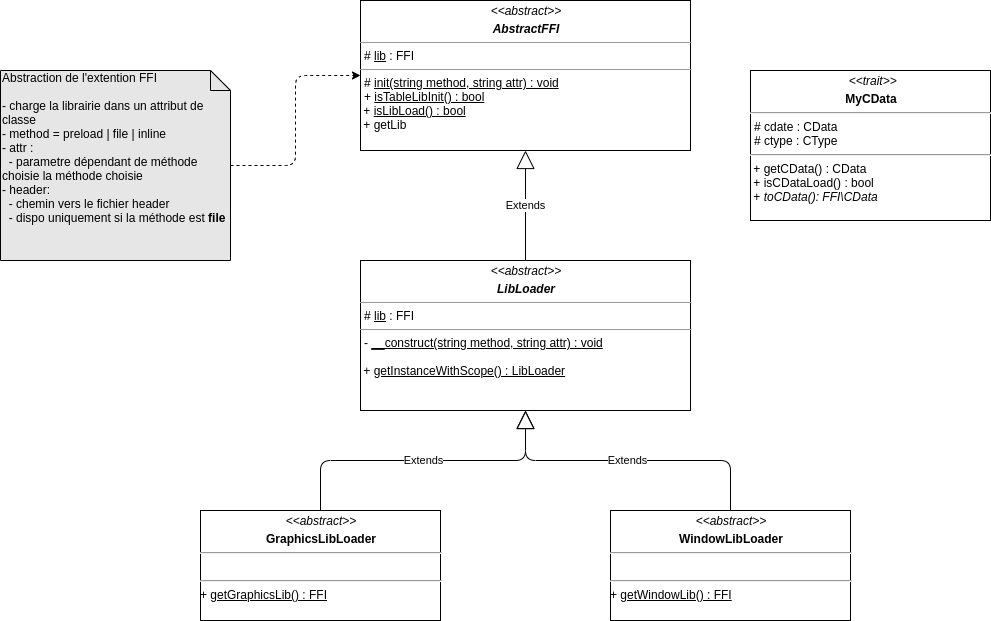
\includegraphics[width=13.76in]{assets/img/class-ffi-abstraction} 

}

\caption{Diagramme de classe : AbstractFFI}\label{fig:class-diagram-abstract-ffi}
\end{figure}

On y voit plusieurs classes abstraites, la principale étant \texttt{AbstractFFI} dont hérite \texttt{LibLoader}, leurs rôles est dans leur nom :

\begin{itemize}
\tightlist
\item
  \textbf{AbstractFFI} : la principale classe qui se charge de s'abstraire du chargement de la bibliothèque et de faire les vérifications nécessaires. Elle a comme attribut un tableau d'objets FFI pour permettre l'utilisation de plusieurs bibliothèque tout au long du programme.
\item
  \textbf{LibLoader} : héritant de AbstractFFI elle a les mêmes fonctionnalités, mais en plus elle donne la base pour mettre en place un Singleton de génération de bibliothèque --- une classe limité à une instance dont le seul objectif est de retourner une bibliothèque précise.
\end{itemize}

Pour ce qui est de \textbf{MyCData}, il s'agit d'un \texttt{trait} --- particularité de PHP, c'est simplement une classe abstraite qui s'utilise comme une interface pour faire simple. Son objectifs est d'avoir un ensemble de fonctions et d'attribut prêtes à être réutiliser pour définir une donnée C qui serait importer de la bibliothèque chargé avec FFI.

\hypertarget{architecture-globale}{%
\subsection{Architecture globale}\label{architecture-globale}}

Le reste de la bibliothèque est un ensemble de classe inspiré de SFML qui s'emboîtent autour de l'abstraction FFI. Effectivement, SFML et pas CSFML, car CSFML est écrit en C, or le C n'est pas un langage orienté objet et CSFML est juste un pont vers SFML qui est écrit en C++ qui lui est bien orienté objet. Toujours est-il que j'ai du simplifier un maximum l'architecture pour ne pas alourdir la bibliothèque en elle même et son utilisation finale.

\hypertarget{exemple-de-la-classe-window}{%
\subsection{Exemple de la classe Window}\label{exemple-de-la-classe-window}}

La classe Window est le deuxième pilier de l'architecture de la bibliothèque, comme la plupart des classes elle utilise MyCData pour bénéficier des méthodes et des attributs lier à l'échange de données entre PHP et la bibliothèque C via FFI. C'est le cas de la méthode \texttt{toCData()} qui convertit les attributs actuel de la classe en donnée C.

\hypertarget{diagramme-de-classe}{%
\subsection{Diagramme de classe}\label{diagramme-de-classe}}

Le résultat de la phase de conception est le diagramme de classe suivant qui a constamment évolué même lors de l'implémentation des fonctionnalités de la bibliothèque.

\label{fig:class-diagramm}Diagramme de classe accessible à l'adresse \url{https://cutt.ly/phpml-class-diagram}

Le temps passé sur la réflexion de l'architecture de la bibliothèque n'a pas été en vain car il va nous permettre d'en gagner sur la partie principale qui est l'implémentation des fonctionnalités trouvées lors de la phase de conception.

\hypertarget{utils}{%
\chapter{Utilisation de la bibliothèque}\label{utils}}

\hypertarget{utils-pre-requis}{%
\section{Pré-requis}\label{utils-pre-requis}}

\hypertarget{res}{%
\chapter{Résultat}\label{res}}

J'ai hâte moi aussi

\hypertarget{exemple-1}{%
\section{Exemple 1}\label{exemple-1}}

\hypertarget{exemple-2}{%
\section{Exemple 2}\label{exemple-2}}

\hypertarget{conclusion}{%
\chapter*{Conclusion}\label{conclusion}}


J'aurai enfin fini\ldots{}

\hypertarget{liste-des-abbreviations}{%
\chapter*{Liste des Abbreviations}\label{liste-des-abbreviations}}


\begin{description}
\item[POO]
Programmation Orientée Objets

La programmation orientée objet (POO), ou programmation par objet, est un paradigme de programmation informatique. Il consiste en la définition et l'interaction de briques logicielles appelées objets ; un objet représente un concept, une idée ou toute entité du monde physique, comme une voiture, une personne ou encore une page d'un livre.

--- \citep{wikipedia_programmation_2020}
\item[FFI]
Foreign Function Interface

C'est un mécanisme par lequel un programme écrit dans un langage de programmation peut appeler des routines ou utiliser des services écrits dans un autre.
\item[URCA]
Université de Reims Champagne Ardenne
\item[IUT-RCC]
Institut Universitaire de Technologie de Reims-Châlons-Charleville
\end{description}

\backmatter

\bibliography{bib/book.bib,bib/citations.bib,packages.bib}

\printindex

\end{document}
